\begin{frame}{Architecture générale}
    \begin{figure}
        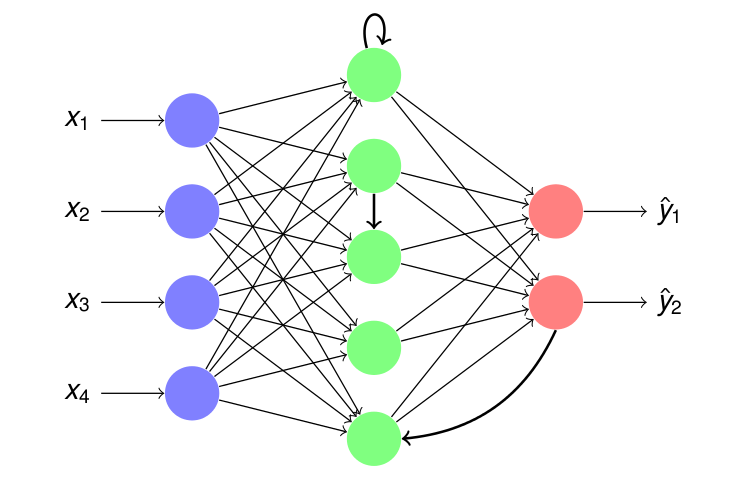
\includegraphics[height=.75\textheight,width=\textwidth,keepaspectratio]{images/arch_rnn_1}
        \caption{Réseau de neurones récurrent {\scriptsize\it -- Source : Cours R. \textsc{Hérault} \& P. \textsc{Leray}}}
    \end{figure}

\end{frame}

\begin{frame}{Architecture d'un RNN d'Elman}
    \begin{figure}
        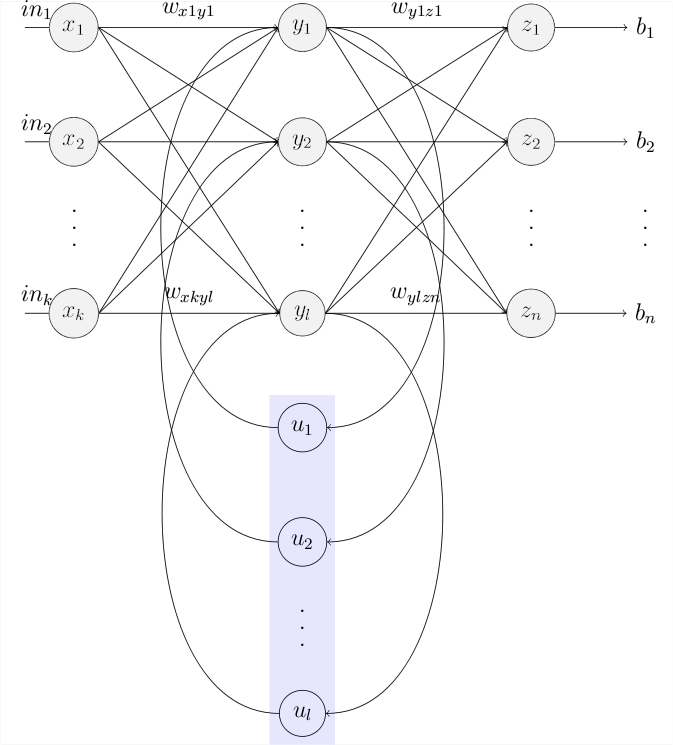
\includegraphics[height=.65\textheight,width=\textwidth,keepaspectratio]{images/Elman_srnn}
        \caption{RNN d'Elman {\scriptsize\it -- Source : wikimedia.org}}
    \end{figure}
    \vspace{-.5cm}
	\begin{itemize} 
		\item La couche $u_1 ... u_n$ sert de mémoire pour l'état précédent 
	\end{itemize}
\end{frame}
